\documentclass[13pt]{beamer}

\usepackage{pgfpages}
\usepackage{minted}
\usepackage[T1]{fontenc}
\usepackage{lmodern}
\usepackage[english]{babel}
\usepackage[utf8x]{inputenc}
\usepackage{graphicx}
\usetheme{default} % or try Darmstadt, Madrid, Warsaw, ...
\usecolortheme{default} % or try albatross, beaver, crane, ...
\usefonttheme{default} % or try serif, structurebold, ...
\setbeamertemplate{navigation symbols}{}
\setbeamertemplate{caption}[numbered]


% For presenter notes
\setbeameroption{show notes on second screen}


\addtobeamertemplate{navigation symbols}{}{%
  \usebeamerfont{footline}%
  \usebeamercolor[fg]{footline}%
  \hspace{1em}%
  \insertframenumber/\inserttotalframenumber
  }

\newcommand\Wider[2][3em]{%
\makebox[\linewidth][c]{%
  \begin{minipage}{\dimexpr\textwidth+#1\relax}
  \raggedright#2
  \end{minipage}%
  }%
}
  
\title{Generic Functions in Java}
\author{Daniel Reigada - 82064}
\institute{IST - Advanced Programming}
% \date{Date of Presentation}

\begin{document}

\begin{frame}
  \titlepage
  \note{
    I will start by presenting how I implemented my solution and then I will show the extensions I've made
  }
\end{frame}

\section{Introduction}

\begin{frame}{Setup on class load (Javassist Translator)}
  \note{
    Starting with the class loader Translator, since writing javassist is error-prone,
    i've decided to put most logic in an helper class that is called from the javassist code
    \begin{enumerate}
      \item Add field with helper object
      \item Rename all functions
      \item Create new methods in with the old name of the renamed ones that only call the helper object
    \end{enumerate}
    
    Renaming the functions instead of using an Expression editor:
    the overhead only happens when the class is loaded insted of when a class that calls the method is loaded
  }

  \begin{enumerate}
    \item Add field with helper object
    \item Rename all functions
    \item Create new methods in place of the renamed ones that only call the helper object.
  \end{enumerate}

\end{frame}

\begin{frame}{Method call}
  \begin{figure}
    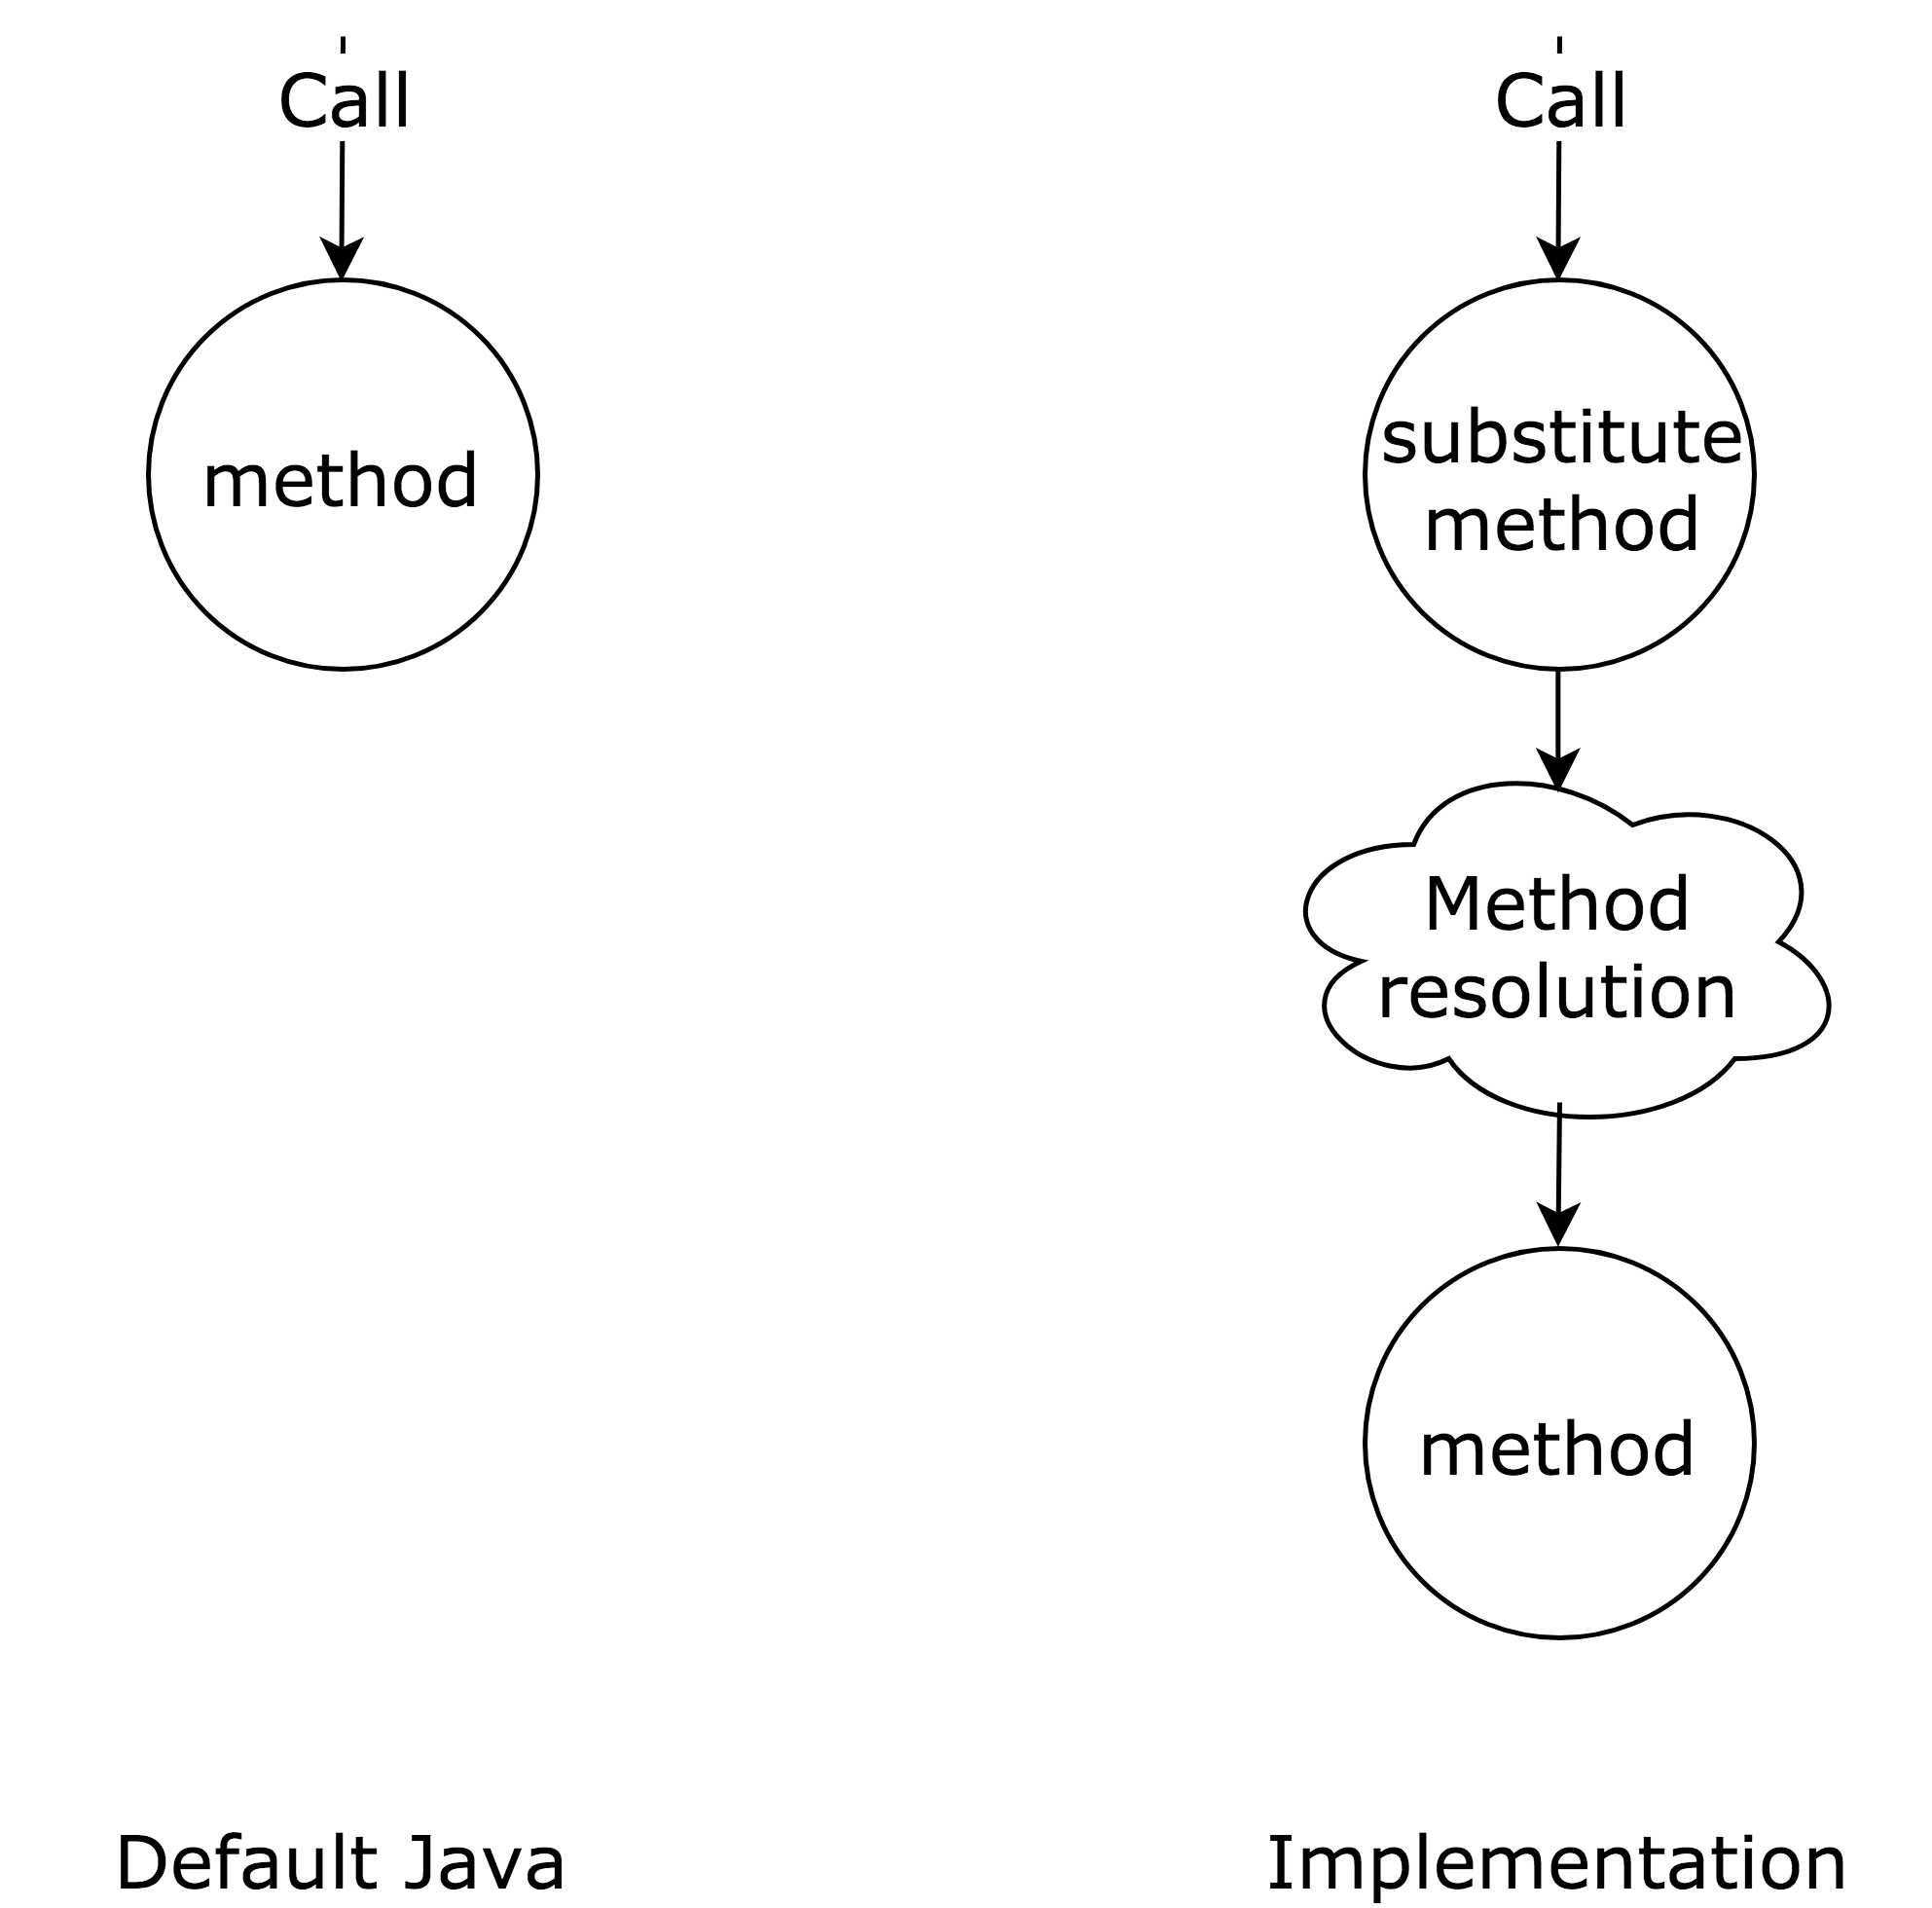
\includegraphics[height=0.78\textheight]{figures/callChain.png}
  \end{figure}
\end{frame}

\begin{frame}{Method resolution}
  \note{ 
    \begin{enumerate}
      \item When the helper class is instantiated a mapping\
        between argument types and applicable methods is generated (to create a cache)
      \item When a method is invoked: {
        \begin{enumerate}
          \item Filter methods applicable to the given arguments 
          \item Sort them by specifity
          \item Invoke the most specific
        \end{enumerate}
      }
    \end{enumerate}
  }

  \begin{enumerate}
    \item When the helper class is instantiated a mapping\
      between argument types and methods is created
    \item When a method is invoked: {
      \begin{enumerate}
        \item Filter methods applicable to the given arguments 
        \item Sort them by specifity
        \item Invoke the most specific
      \end{enumerate}
    }
  \end{enumerate}
\end{frame}

\begin{frame}{Extensions}
  \note{
    I've implemented two extensions, method caching and custom method order
  }
  \begin{itemize}
    \item Method caching
    \item Allowing custom ordering of methods
  \end{itemize}
\end{frame}

\begin{frame}{Cache Comparison}
  \note{
    Method caching is not that interesting but it has a huge improvement in performance
    
    For normal java we can see that the JIT compiler optimizes the calls really well
    
    But if we compare the cache version with the normal one we see that the improvements are much more significant
    
    Almost two orders of magnitude faster when making a million calls
  }

    \begin{table}[]
      \centering
      \resizebox{\textwidth}{!}{
        \begin{tabular}{llllll}
                    & 1    & 10 000 & 100 000 & 1 000 000 &  \\
        No cache    & 154  & 156.8 & 830.8  & 7929.7  &  \\
        With cache  & 27.4 & 25.1  & 49.8   & 130.9   &  \\
        Java        & 0.2  & 0.6   & 0.7    & 0.4     & 
        \end{tabular}
      }
      \caption{Time comparison by the number of function calls (milliseconds)}
      \label{comparison-table}
      \end{table}
\end{frame}

\begin{frame}[fragile]{Custom Method Ordering (Comparator)}
  \note {
    With the second extension, we can define a custom way of ordering methods
    We just need to implement an MethodComparator
    
    In this useless example we just reverse the default order of methods,
    except if the first argument of the method is Object
  }
  \begin{minted}[fontsize=\footnotesize]{java}
    public class ReversedComparator extends AbstractMethodComparator {
      /* ... */

      @Override
      public int compare(Method m1, Method m2) {
        boolean m1FirstIsObject =
          m1.getParameterTypes()[0].equals(Object.class);
        boolean m2FirstIsObject =
          m2.getParameterTypes()[0].equals(Object.class);

        if (m1FirstIsObject && !m2FirstIsObject) {
          return 1;
        } else if (!m1FirstIsObject && m2FirstIsObject) {
          return -1;
        } else {
          return defaultComp.reversed().compare(m1, m2);
        }
      }
    }
  \end{minted}
\end{frame}

\begin{frame}[fragile]{Custom Method Ordering (Generic Function)}
  \note{
    Here we implement the Generic Function with the extension parameters
  }
  \begin{minted}[fontsize=\footnotesize]{java}
    @GenericFunctionExtended(
      useCache = false,
      methodComparator = ReversedComparator.class)
      public interface Rever {
        static String sed(Object o) { return "Object"; }
      
        static String sed(MyInterface1 o) { return "MyInterface1"; }
    
        static String sed(MyClass1 o) { return "MyClass1"; }

        static String sed(MyClass2 o) { return "MyClass2"; }
      }
  \end{minted}
\end{frame}

\begin{frame}[fragile]{Custom Method Ordering}
  \note{
    And then we call the functions

    Since we reversed the default order of methods we can see that in the first example the function that takes the interface as a parameter is called
    (but not the one that is defined for Object)
  }
  
  \begin{minted}[fontsize=\footnotesize]{java}
    interface MyInterface1 {}
    class MyClass1 implements MyInterface1 {}
    
    class MyClass2 {}
  \end{minted}

  \vspace{5mm} %5mm vertical space

  \begin{minted}[fontsize=\footnotesize]{java}
    Rever.sed((Object) new MyClass1());
    // "MyInterface1"
    Rever.sed((Object) new MyClass2());
    // "MyClass2"
  \end{minted}
\end{frame}

\end{document}
